\section{Fault-Tolerance Mechanisms}
This section covers some mechanisms which can improve fault-tolerance in
microservice architectures. Their functionality and intended purpose will
be covered in this section, and their implementation will be covered in 
Section~\ref{sec:implementation}.

\subsection{Timeouts}

\subsection{Bulkheads}

\subsection{Circuit Breaker}
Since microservices typically rely on networked interprocess communication,
there is a risk of calls between them failing or hanging with no timely
response.
If a service relies on another service which starts failing, resulting in not
responding and letting requests hang, the requesting service can waste its
resources on threads waiting for responses. Other than affecting the requesting
services interaction with the failing service, it might also take its resources
from serving its own functionality to other services. This can result in
cascading failures throughout a system~\cite{fowler2014blog}.
Failures can be anything from requests timing out, $5xx HTTP$ responses to
overflowing message queues. 
\newline\newline
The \textit{Circuit Breaker} pattern was introduced by Michael
Nygard~\cite{nygard2007release}, and solves the problem of resource exhaustion
caused by requests to failing services, by failing quickly if it is observed
that requests to a service fail frequently. 
This is achieved by wrapping all calls/requests to a service in a
\textit{circuit breaker} object, which monitors the interaction for continuous
number of failures. 
If the number of failing requests reach some predefined threshold, the circuit
is opened. 
\newline\newline
When in the \textit{open} state, requests will fail immediately instead of being
forwarded, hereby minimizing the number of threads waiting for responses and
allowing the requested service to recover from whatever has caused it to fail.
After some defined timeout, the circuit will transition to a \textit{half-open}
state, where requests will be let through to the service, to see if it functions
again. If it functions as expected, the circuit will be opened again, if not it
will go back to its \textit{closed} state again. This is illustrated as a state
machine in Figure~\ref{fig:circuitbreakerstate}.

\begin{figure}[H]
\centering
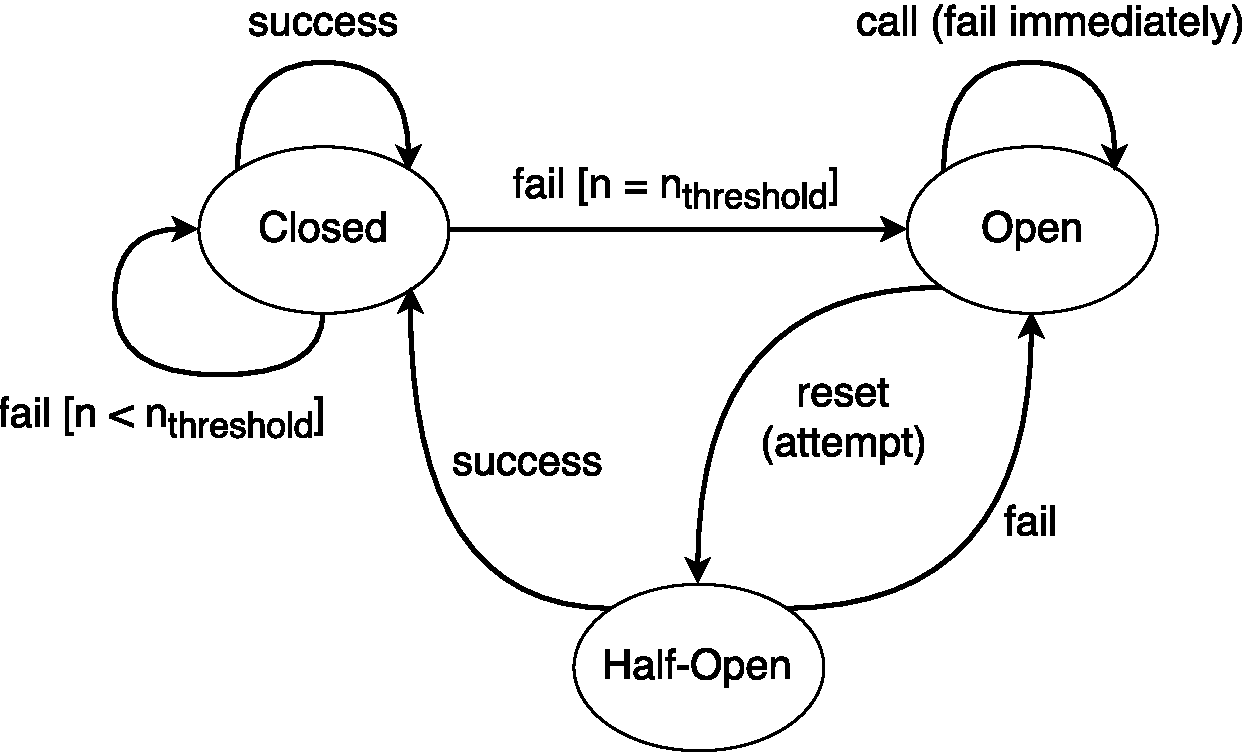
\includegraphics[width=0.7\textwidth]{../media/CircuitBreakerState.pdf} 
\caption{State machine representing the \textit{circuit breaker}. The
	circuit can be in states \textit{closed}, \textit{open} or \textit{half-open}.
	The circuit will transition to its \textit{open} state if number of continuous
	failures reach a predefined threshold. Circuit will be in \textit{closed}
	state until it reaches a timeout where it will reset itself to the
	\textit{half-open} state, from where it will either transition to
	\textit{closed} if a request succeeds or to \textit{open} if a request fails.}
\label{fig:circuitbreakerstate}
\end{figure}

\subsection{Replication}
% Replication of stateless services, split workload
One key principle of microservices, is the componentization of software in
independent services. If they are implemented in a stateless manner, only
persisting state in databases, the independent services can be replicated and
function side-by-side, hereby splitting the system load. Which in many cases
might also minimize errors, since overloading a service could cause faults.
Beyond allowing a service to be scaled horizontally, replication also allows
for increased fault-tolerance, since the failure of a single instance does not
necessarily result in breaking the system, since other identical replicated
services are still running. The key goal being that at least one instance of the
service is alive, reachable and well-behaved.
\newline\newline
Replication can enhance fault-tolerance even more, if it is applied on a cluster
of servers. Replicating services across a cluster, spreading replicas to
different nodes, lets the system handle sudden disconnects or downtime on
individual nodes. This mentality can even be applied on datacenters and the
cloud, where a single system might run replicated on datacenters and clouds
from different providers and across different regions.
\newline\newline
Another benefit of replication is the ability to deploy a new version of a
service one replica at a time. This allows for evaluation of its performance
in a system and quick rollback if faults are encountered, with no downtime.

\subsection{Redundancy}
% Multiple hosts and services ready for fail-over

\subsection{Resilience}
% Self healing of Docker Swarm orchestration

